% Options for packages loaded elsewhere
% Options for packages loaded elsewhere
\PassOptionsToPackage{unicode}{hyperref}
\PassOptionsToPackage{hyphens}{url}
\PassOptionsToPackage{dvipsnames,svgnames,x11names}{xcolor}
%
\documentclass[
  11pt,
]{article}
\usepackage{xcolor}
\usepackage[margin=1in]{geometry}
\usepackage{amsmath,amssymb}
\setcounter{secnumdepth}{-\maxdimen} % remove section numbering
\usepackage{iftex}
\ifPDFTeX
  \usepackage[T1]{fontenc}
  \usepackage[utf8]{inputenc}
  \usepackage{textcomp} % provide euro and other symbols
\else % if luatex or xetex
  \usepackage{unicode-math} % this also loads fontspec
  \defaultfontfeatures{Scale=MatchLowercase}
  \defaultfontfeatures[\rmfamily]{Ligatures=TeX,Scale=1}
\fi
\usepackage{lmodern}
\ifPDFTeX\else
  % xetex/luatex font selection
\fi
% Use upquote if available, for straight quotes in verbatim environments
\IfFileExists{upquote.sty}{\usepackage{upquote}}{}
\IfFileExists{microtype.sty}{% use microtype if available
  \usepackage[]{microtype}
  \UseMicrotypeSet[protrusion]{basicmath} % disable protrusion for tt fonts
}{}
\makeatletter
\@ifundefined{KOMAClassName}{% if non-KOMA class
  \IfFileExists{parskip.sty}{%
    \usepackage{parskip}
  }{% else
    \setlength{\parindent}{0pt}
    \setlength{\parskip}{6pt plus 2pt minus 1pt}}
}{% if KOMA class
  \KOMAoptions{parskip=half}}
\makeatother
% Make \paragraph and \subparagraph free-standing
\makeatletter
\ifx\paragraph\undefined\else
  \let\oldparagraph\paragraph
  \renewcommand{\paragraph}{
    \@ifstar
      \xxxParagraphStar
      \xxxParagraphNoStar
  }
  \newcommand{\xxxParagraphStar}[1]{\oldparagraph*{#1}\mbox{}}
  \newcommand{\xxxParagraphNoStar}[1]{\oldparagraph{#1}\mbox{}}
\fi
\ifx\subparagraph\undefined\else
  \let\oldsubparagraph\subparagraph
  \renewcommand{\subparagraph}{
    \@ifstar
      \xxxSubParagraphStar
      \xxxSubParagraphNoStar
  }
  \newcommand{\xxxSubParagraphStar}[1]{\oldsubparagraph*{#1}\mbox{}}
  \newcommand{\xxxSubParagraphNoStar}[1]{\oldsubparagraph{#1}\mbox{}}
\fi
\makeatother


\usepackage{longtable,booktabs,array}
\newcounter{none} % for unnumbered tables
\usepackage{calc} % for calculating minipage widths
% Correct order of tables after \paragraph or \subparagraph
\usepackage{etoolbox}
\makeatletter
\patchcmd\longtable{\par}{\if@noskipsec\mbox{}\fi\par}{}{}
\makeatother
% Allow footnotes in longtable head/foot
\IfFileExists{footnotehyper.sty}{\usepackage{footnotehyper}}{\usepackage{footnote}}
\makesavenoteenv{longtable}
\usepackage{graphicx}
\makeatletter
\newsavebox\pandoc@box
\newcommand*\pandocbounded[1]{% scales image to fit in text height/width
  \sbox\pandoc@box{#1}%
  \Gscale@div\@tempa{\textheight}{\dimexpr\ht\pandoc@box+\dp\pandoc@box\relax}%
  \Gscale@div\@tempb{\linewidth}{\wd\pandoc@box}%
  \ifdim\@tempb\p@<\@tempa\p@\let\@tempa\@tempb\fi% select the smaller of both
  \ifdim\@tempa\p@<\p@\scalebox{\@tempa}{\usebox\pandoc@box}%
  \else\usebox{\pandoc@box}%
  \fi%
}
% Set default figure placement to htbp
\def\fps@figure{htbp}
\makeatother





\setlength{\emergencystretch}{3em} % prevent overfull lines

\providecommand{\tightlist}{%
  \setlength{\itemsep}{0pt}\setlength{\parskip}{0pt}}



 


\usepackage{float}
\makeatletter
\@ifpackageloaded{caption}{}{\usepackage{caption}}
\AtBeginDocument{%
\ifdefined\contentsname
  \renewcommand*\contentsname{Table of contents}
\else
  \newcommand\contentsname{Table of contents}
\fi
\ifdefined\listfigurename
  \renewcommand*\listfigurename{List of Figures}
\else
  \newcommand\listfigurename{List of Figures}
\fi
\ifdefined\listtablename
  \renewcommand*\listtablename{List of Tables}
\else
  \newcommand\listtablename{List of Tables}
\fi
\ifdefined\figurename
  \renewcommand*\figurename{Figure}
\else
  \newcommand\figurename{Figure}
\fi
\ifdefined\tablename
  \renewcommand*\tablename{Table}
\else
  \newcommand\tablename{Table}
\fi
}
\@ifpackageloaded{float}{}{\usepackage{float}}
\floatstyle{ruled}
\@ifundefined{c@chapter}{\newfloat{codelisting}{h}{lop}}{\newfloat{codelisting}{h}{lop}[chapter]}
\floatname{codelisting}{Listing}
\newcommand*\listoflistings{\listof{codelisting}{List of Listings}}
\makeatother
\makeatletter
\makeatother
\makeatletter
\@ifpackageloaded{caption}{}{\usepackage{caption}}
\@ifpackageloaded{subcaption}{}{\usepackage{subcaption}}
\makeatother
\usepackage{bookmark}
\IfFileExists{xurl.sty}{\usepackage{xurl}}{} % add URL line breaks if available
\urlstyle{same}
% fallback for those not using the hyperref driver hyperxmp:
\makeatletter
\@ifundefined{xmpquote}{\newcommand{\xmpquote}[1]{#1}}{}
\makeatother
\hypersetup{
  pdftitle={Problem Set 2},
  pdfauthor={Helena, Igor, and Qixuan},
  colorlinks=true,
  linkcolor={blue},
  filecolor={Maroon},
  citecolor={Blue},
  urlcolor={Blue},
  pdfcreator={LaTeX via pandoc}}


\title{Problem Set 2}
\usepackage{etoolbox}
\makeatletter
\providecommand{\subtitle}[1]{% add subtitle to \maketitle
  \apptocmd{\@title}{\par {\large #1 \par}}{}{}
}
\makeatother
\subtitle{Industrial Organization}
\author{Helena, Igor, and Qixuan}
\date{2026-10-20}
\begin{document}
\maketitle


\subsection{Part 0: Empirical Target}\label{part-0-empirical-target}

\subsubsection{Object of Interest}\label{object-of-interest}

Our main empirical objective is to
\textbf{quantify the welfare gains associated with the availability of gluten-free noodle options on college campuses}.
Specifically, we aim to estimate the change in student welfare relative
to a counterfactual market in which none of the chains offers
gluten-free options. In addition to estimating the average welfare gain
across students, we aim to characterize how these gains vary across
student groups, particularly athletes and graduate students.

More precisely, our object of interest is the change in consumer surplus
resulting from the introduction of gluten-free options, both on average
and separately across groups defined by students' observable
characteristics. This allows us to assess not only the overall benefits
of expanding the available choice set, but also how these benefits are
distributed across different types of students.

\subsubsection{Demand Estimation and Consumer
Preferences}\label{demand-estimation-and-consumer-preferences}

To quantify these welfare gains, we will estimate a discrete-choice
demand model based on a random utility framework. Student utility will
depend on product prices and observable characteristics, such as
spiciness, wheat content, the vegetable-to-meat ratio, and calories, as
well as unobserved product and consumer characteristics.

We will begin with the logit specifications in Part II and then allow
for heterogeneous preferences through random-coefficient models in Part
III. These specifications will help us characterize how students trade
off prices and product characteristics, as well as how preferences vary
across students with different observable characteristics, particularly
athletes and graduate students.

\subsubsection{Price Variation and Product
Substitution}\label{price-variation-and-product-substitution}

A key challenge is that observed prices may be endogenous if stores
adjust prices in response to unobserved product attractiveness. We will
therefore investigate whether local input-cost shocks provide suitable
instruments for product prices. Specifically, variation in local prices
of wheat, vegetables, and meat, combined with differences in product
composition, may generate exogenous variation in production costs and
help identify price sensitivity.

We will also characterize substitution patterns across products.
Observed market shares will inform the estimation of demand, while the
hypothetical second-choice responses in the survey can provide
additional information on substitution between alternatives. These data
may improve our understanding of how students would reallocate their
choices if gluten-free products were unavailable.

\subsubsection{Counterfactual and Welfare
Measurement}\label{counterfactual-and-welfare-measurement}

Using the estimated demand model, we will simulate a counterfactual in
which all gluten-free products are removed from the choice set, while
the prices and characteristics of the remaining products are held
constant. Holding the prices of the remaining products fixed is a
simplifying assumption that isolates the direct welfare effect of
expanding the available choice set and facilitates computation. It
abstracts from potential equilibrium price adjustments following the
introduction or removal of gluten-free products.

We will measure welfare changes using the model-implied change in
consumer surplus, accounting for the estimated price sensitivity and,
where applicable, heterogeneity in preferences. Finally, we will examine
heterogeneity in welfare gains across student groups, particularly
athletes and graduate students. Comparing results across the logit and
random-coefficient specifications will allow us to assess how
assumptions about preference heterogeneity affect the estimated benefits
of gluten-free options.

\subsection{Part 1: Empirical Evidence, Early
Exhibits}\label{part-1-empirical-evidence-early-exhibits}

\paragraph{Data Patterns}\label{data-patterns}

Figure 1 documents the evolution of noodle market shares between 2001
and 2020. Traditional noodles account for the majority of the market
before the introduction of gluten-free (GF) options in 2011. Following
their introduction, GF noodles gain market share, with a further
increase around 2016, when additional chains begin offering GF
alternatives. Over the same period, the market share of traditional
noodles declines. These patterns are consistent with a change in the
composition of noodle demand as GF alternatives become available,
although the figure alone cannot establish that their introduction
caused the decline in traditional noodle shares.

Related to that, Figure 2 examines whether GF choices vary across
student groups over time. The share of GF choices increases for both
athletes and non-athletes, as well as for graduate students and
undergraduates, particularly after 2015. The differences between groups
vary across years, suggesting potential heterogeneity in adoption
patterns. However, these comparisons are descriptive and may also
reflect changes in the composition of the surveyed students and campuses
over time.

\begin{figure}[H]

\centering{

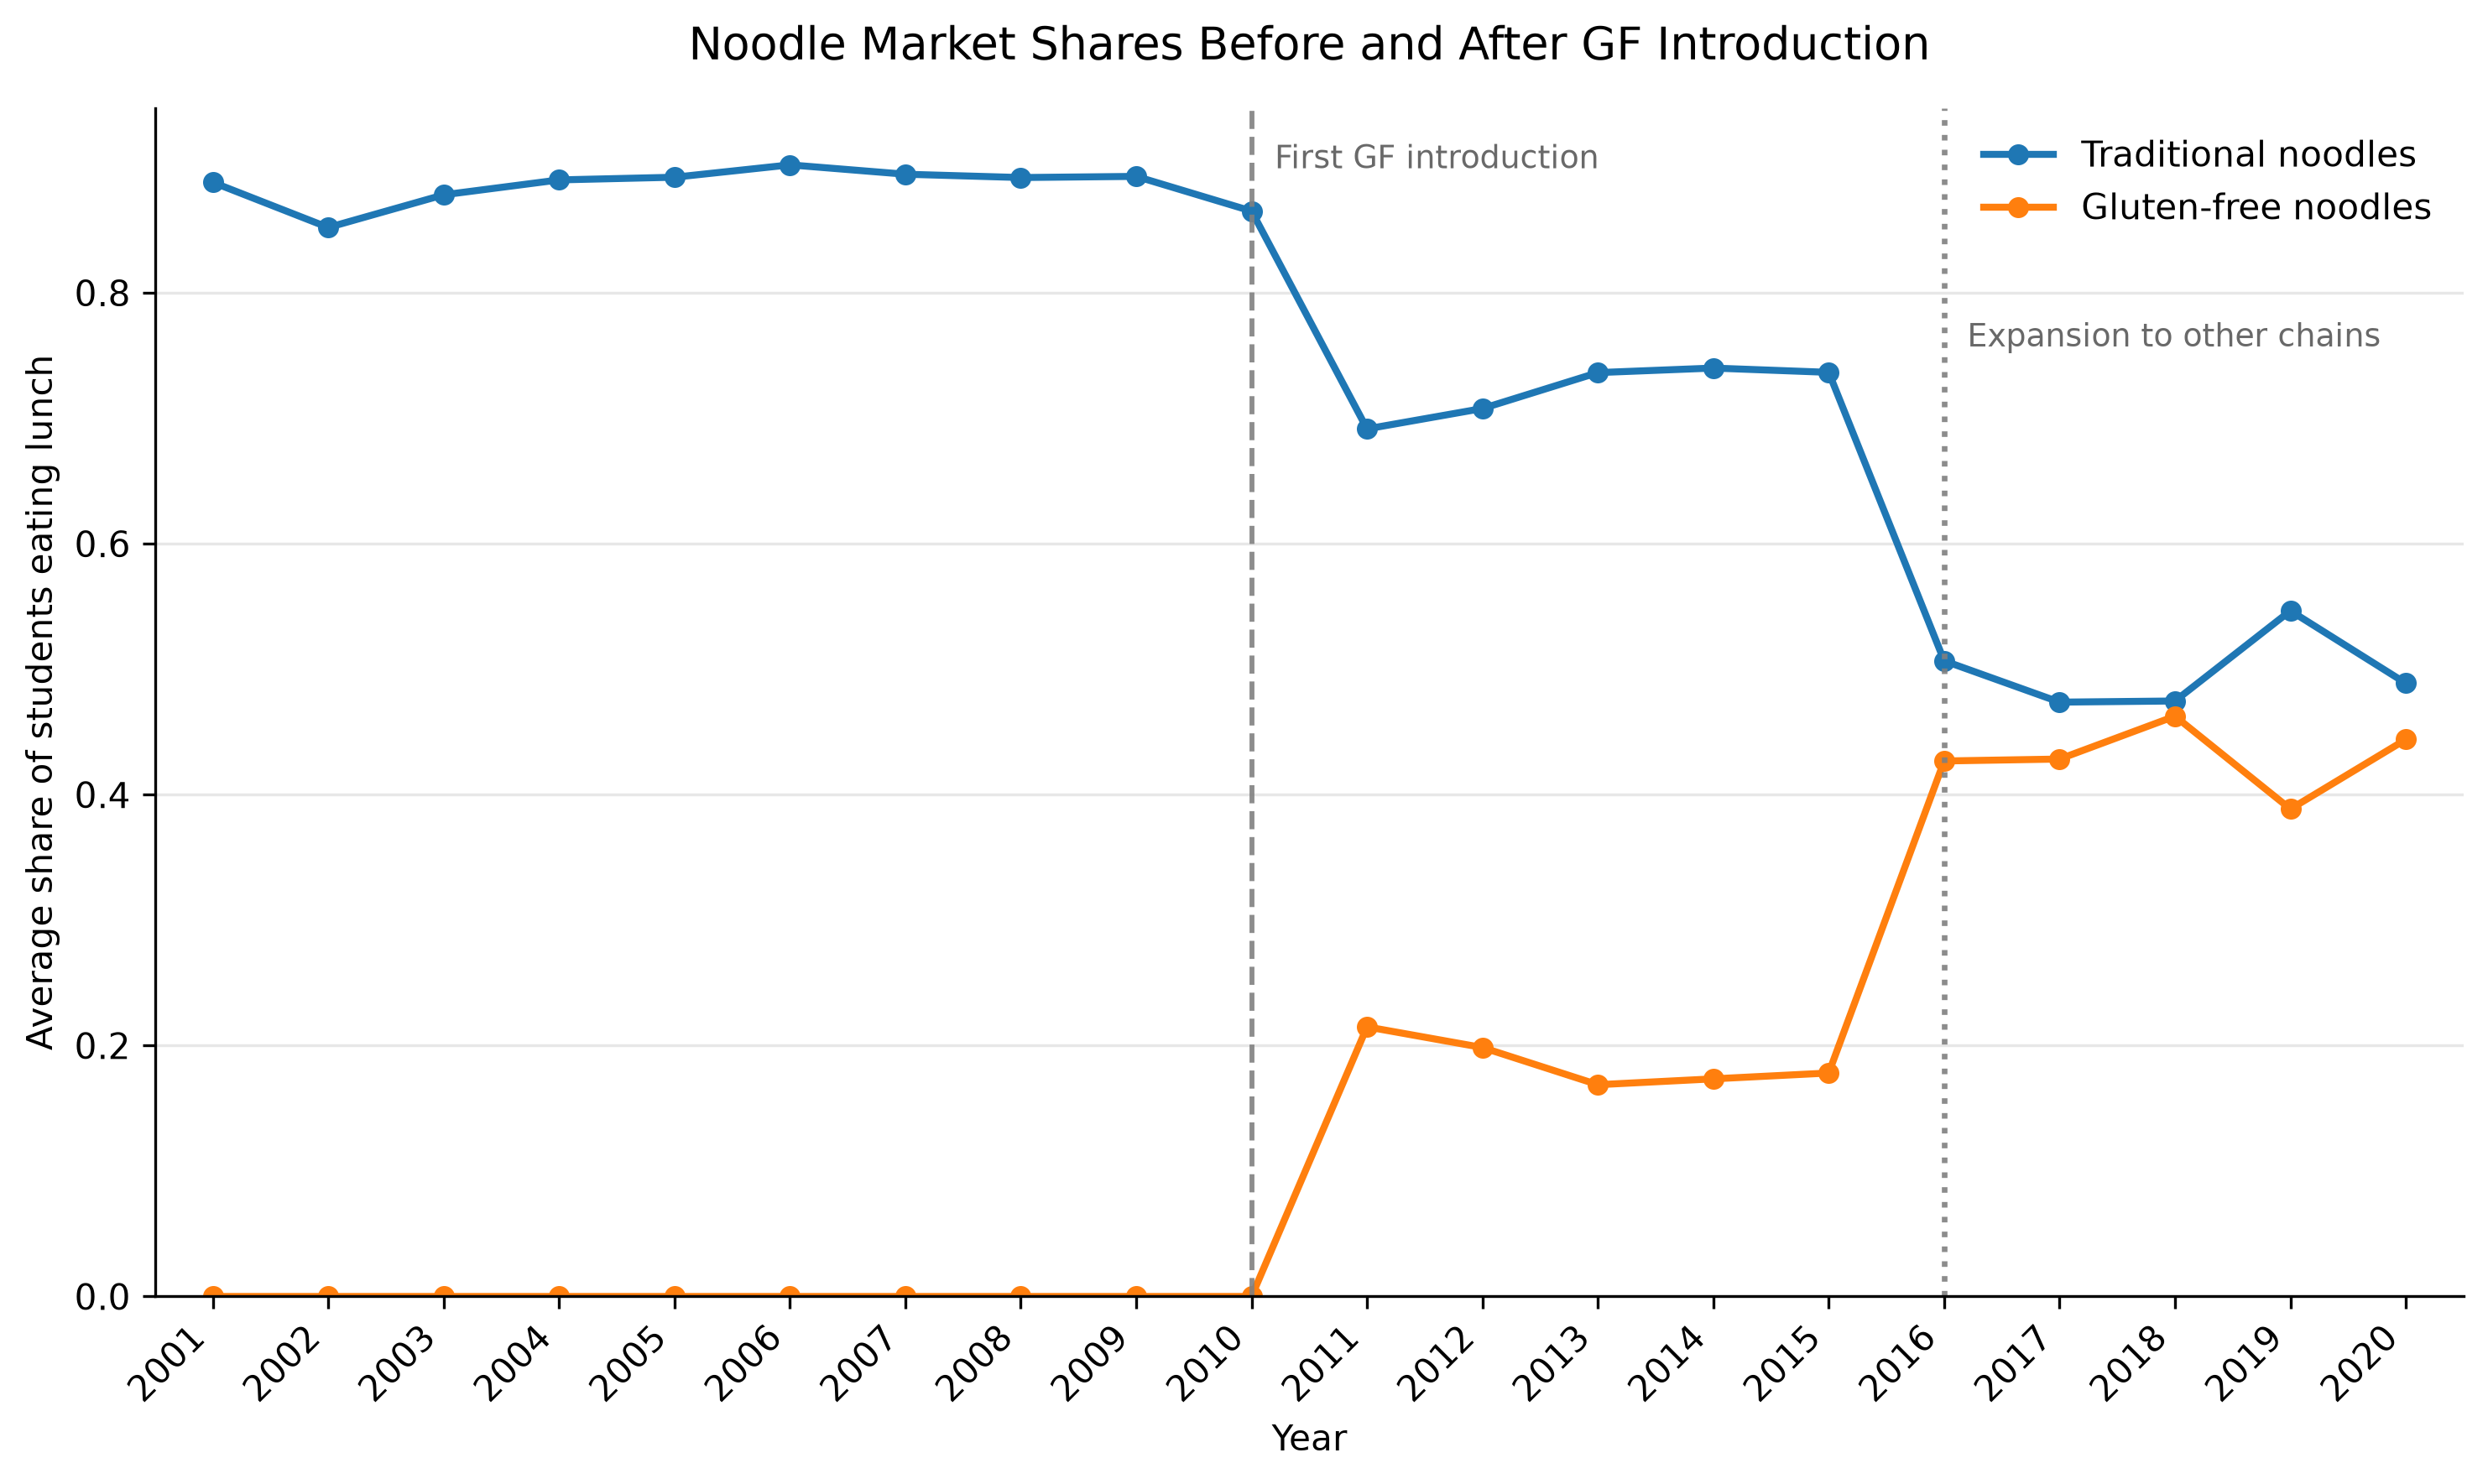
\includegraphics[width=0.9\linewidth,height=\textheight,keepaspectratio]{data/output/evolution_shares.png}

}

\caption{\label{fig-market-shares-evolution}Market shares evolution}

\end{figure}%

\begin{figure}[H]

\centering{

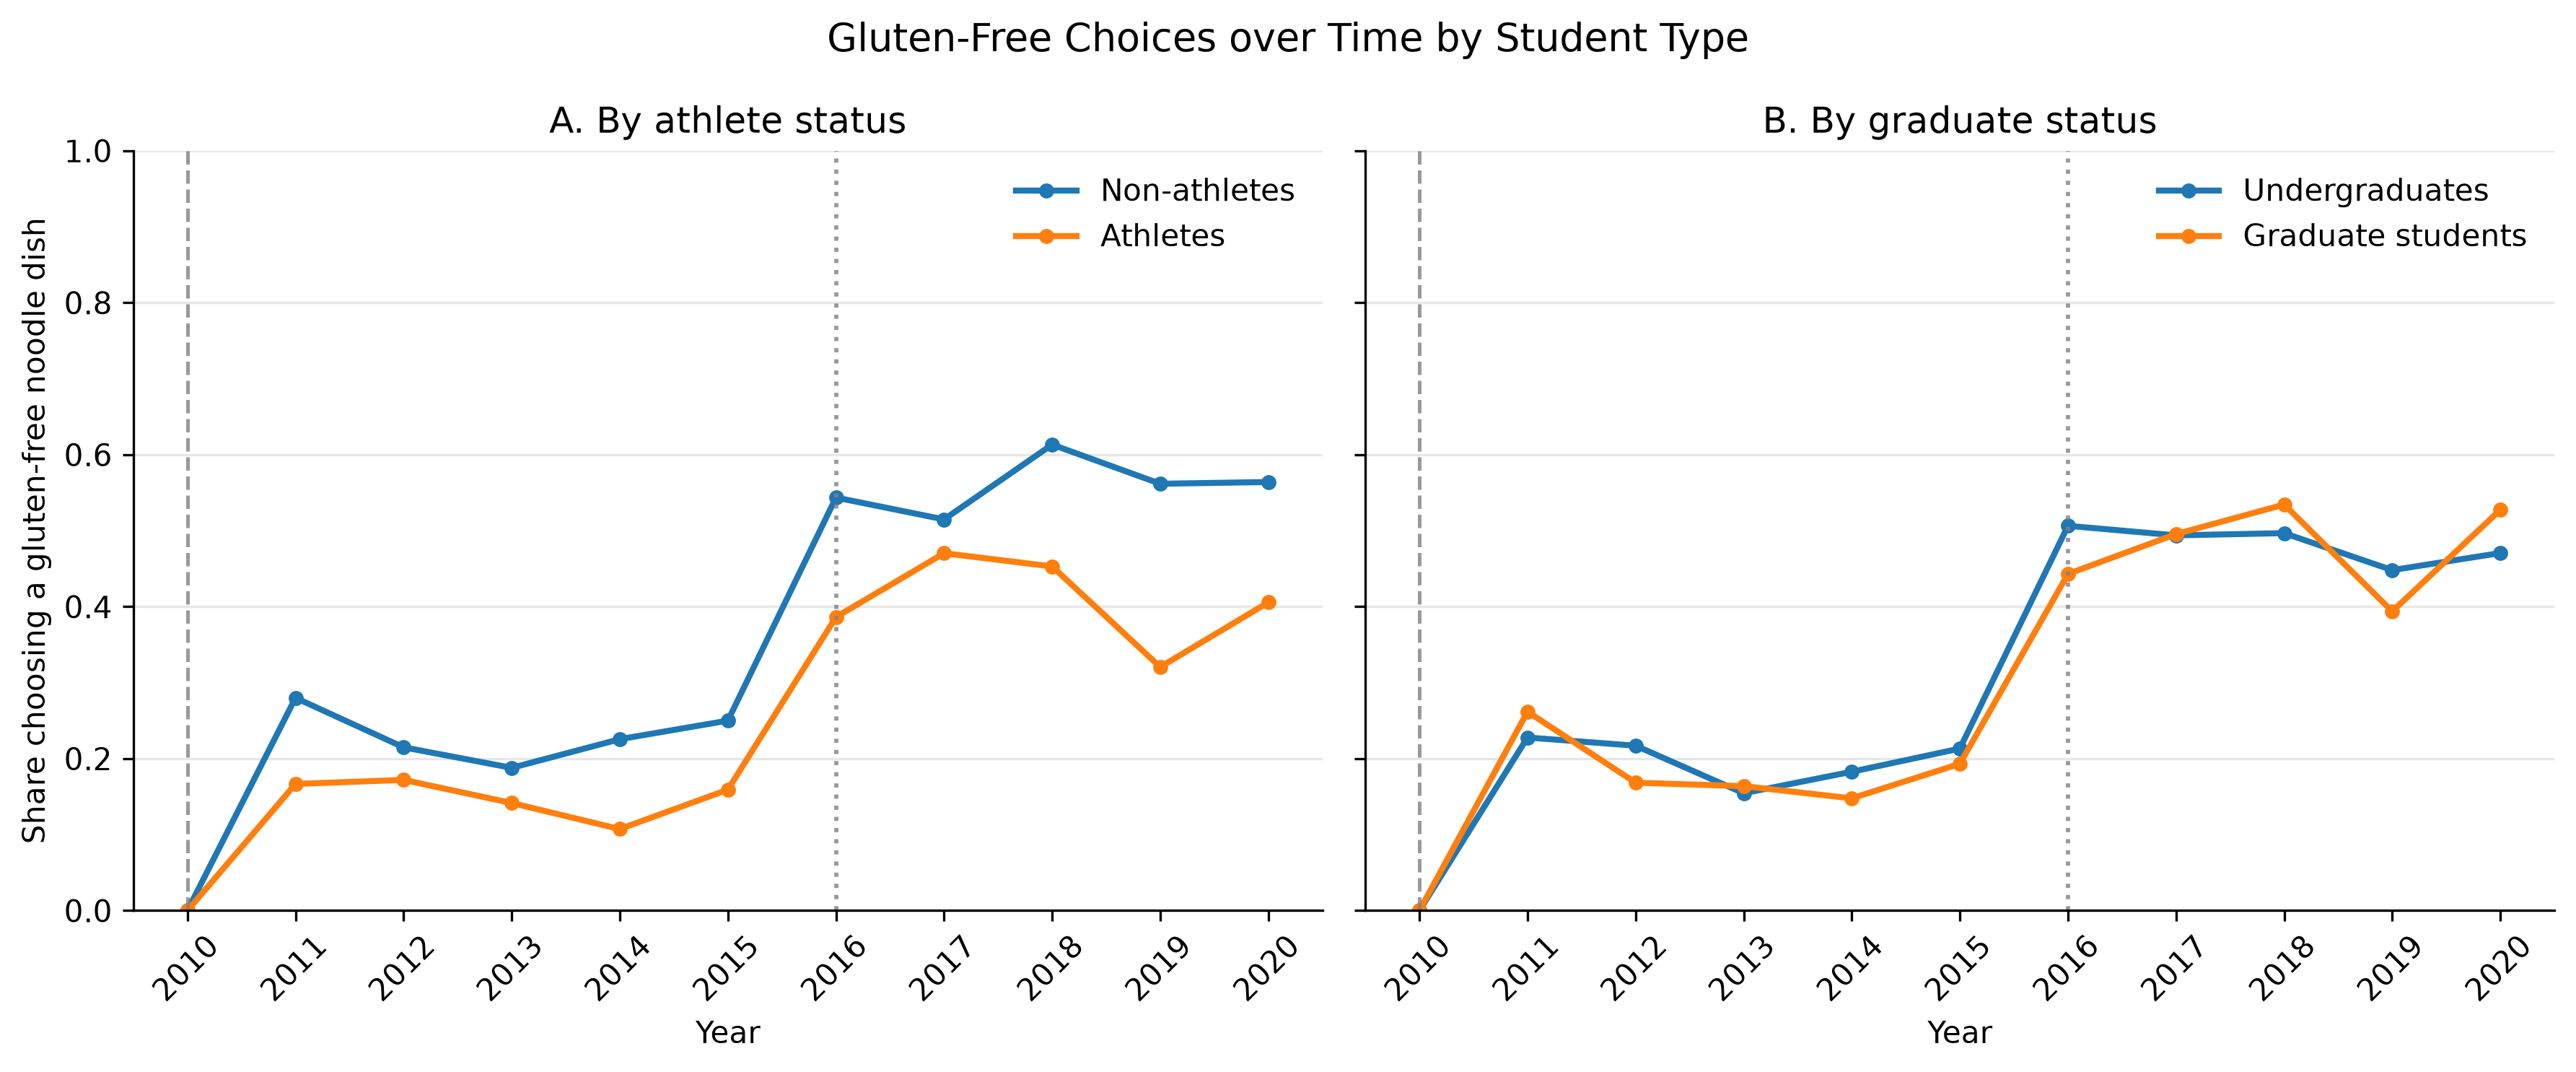
\includegraphics[width=0.9\linewidth,height=\textheight,keepaspectratio]{data/output/choices_bystudent.png}

}

\caption{\label{fig-choices-by-student}Choices by student}

\end{figure}%

Figure 3 presents preliminary dish-specific log-log regression
coefficients relating noodle market shares to own prices, input-price
indices, and the availability of GF alternatives over 2010--2020.
Own-price coefficients are negative for most dishes, indicating a
negative conditional association between prices and market shares. The
coefficients on input-price indices vary across dishes, suggesting that
the relationships between local input costs and product shares are not
uniform. The GF-options coefficients are also heterogeneous: they are
negative for GF dishes and some traditional dishes, but positive for
others. These estimates provide an exploratory description of how market
shares co-vary with prices, costs, and GF availability. They should not
be interpreted as causal effects or structural demand elasticities,
since prices may be endogenous and the regressions do not fully account
for all demand-side and market-level changes.

\begin{figure}[H]

\centering{

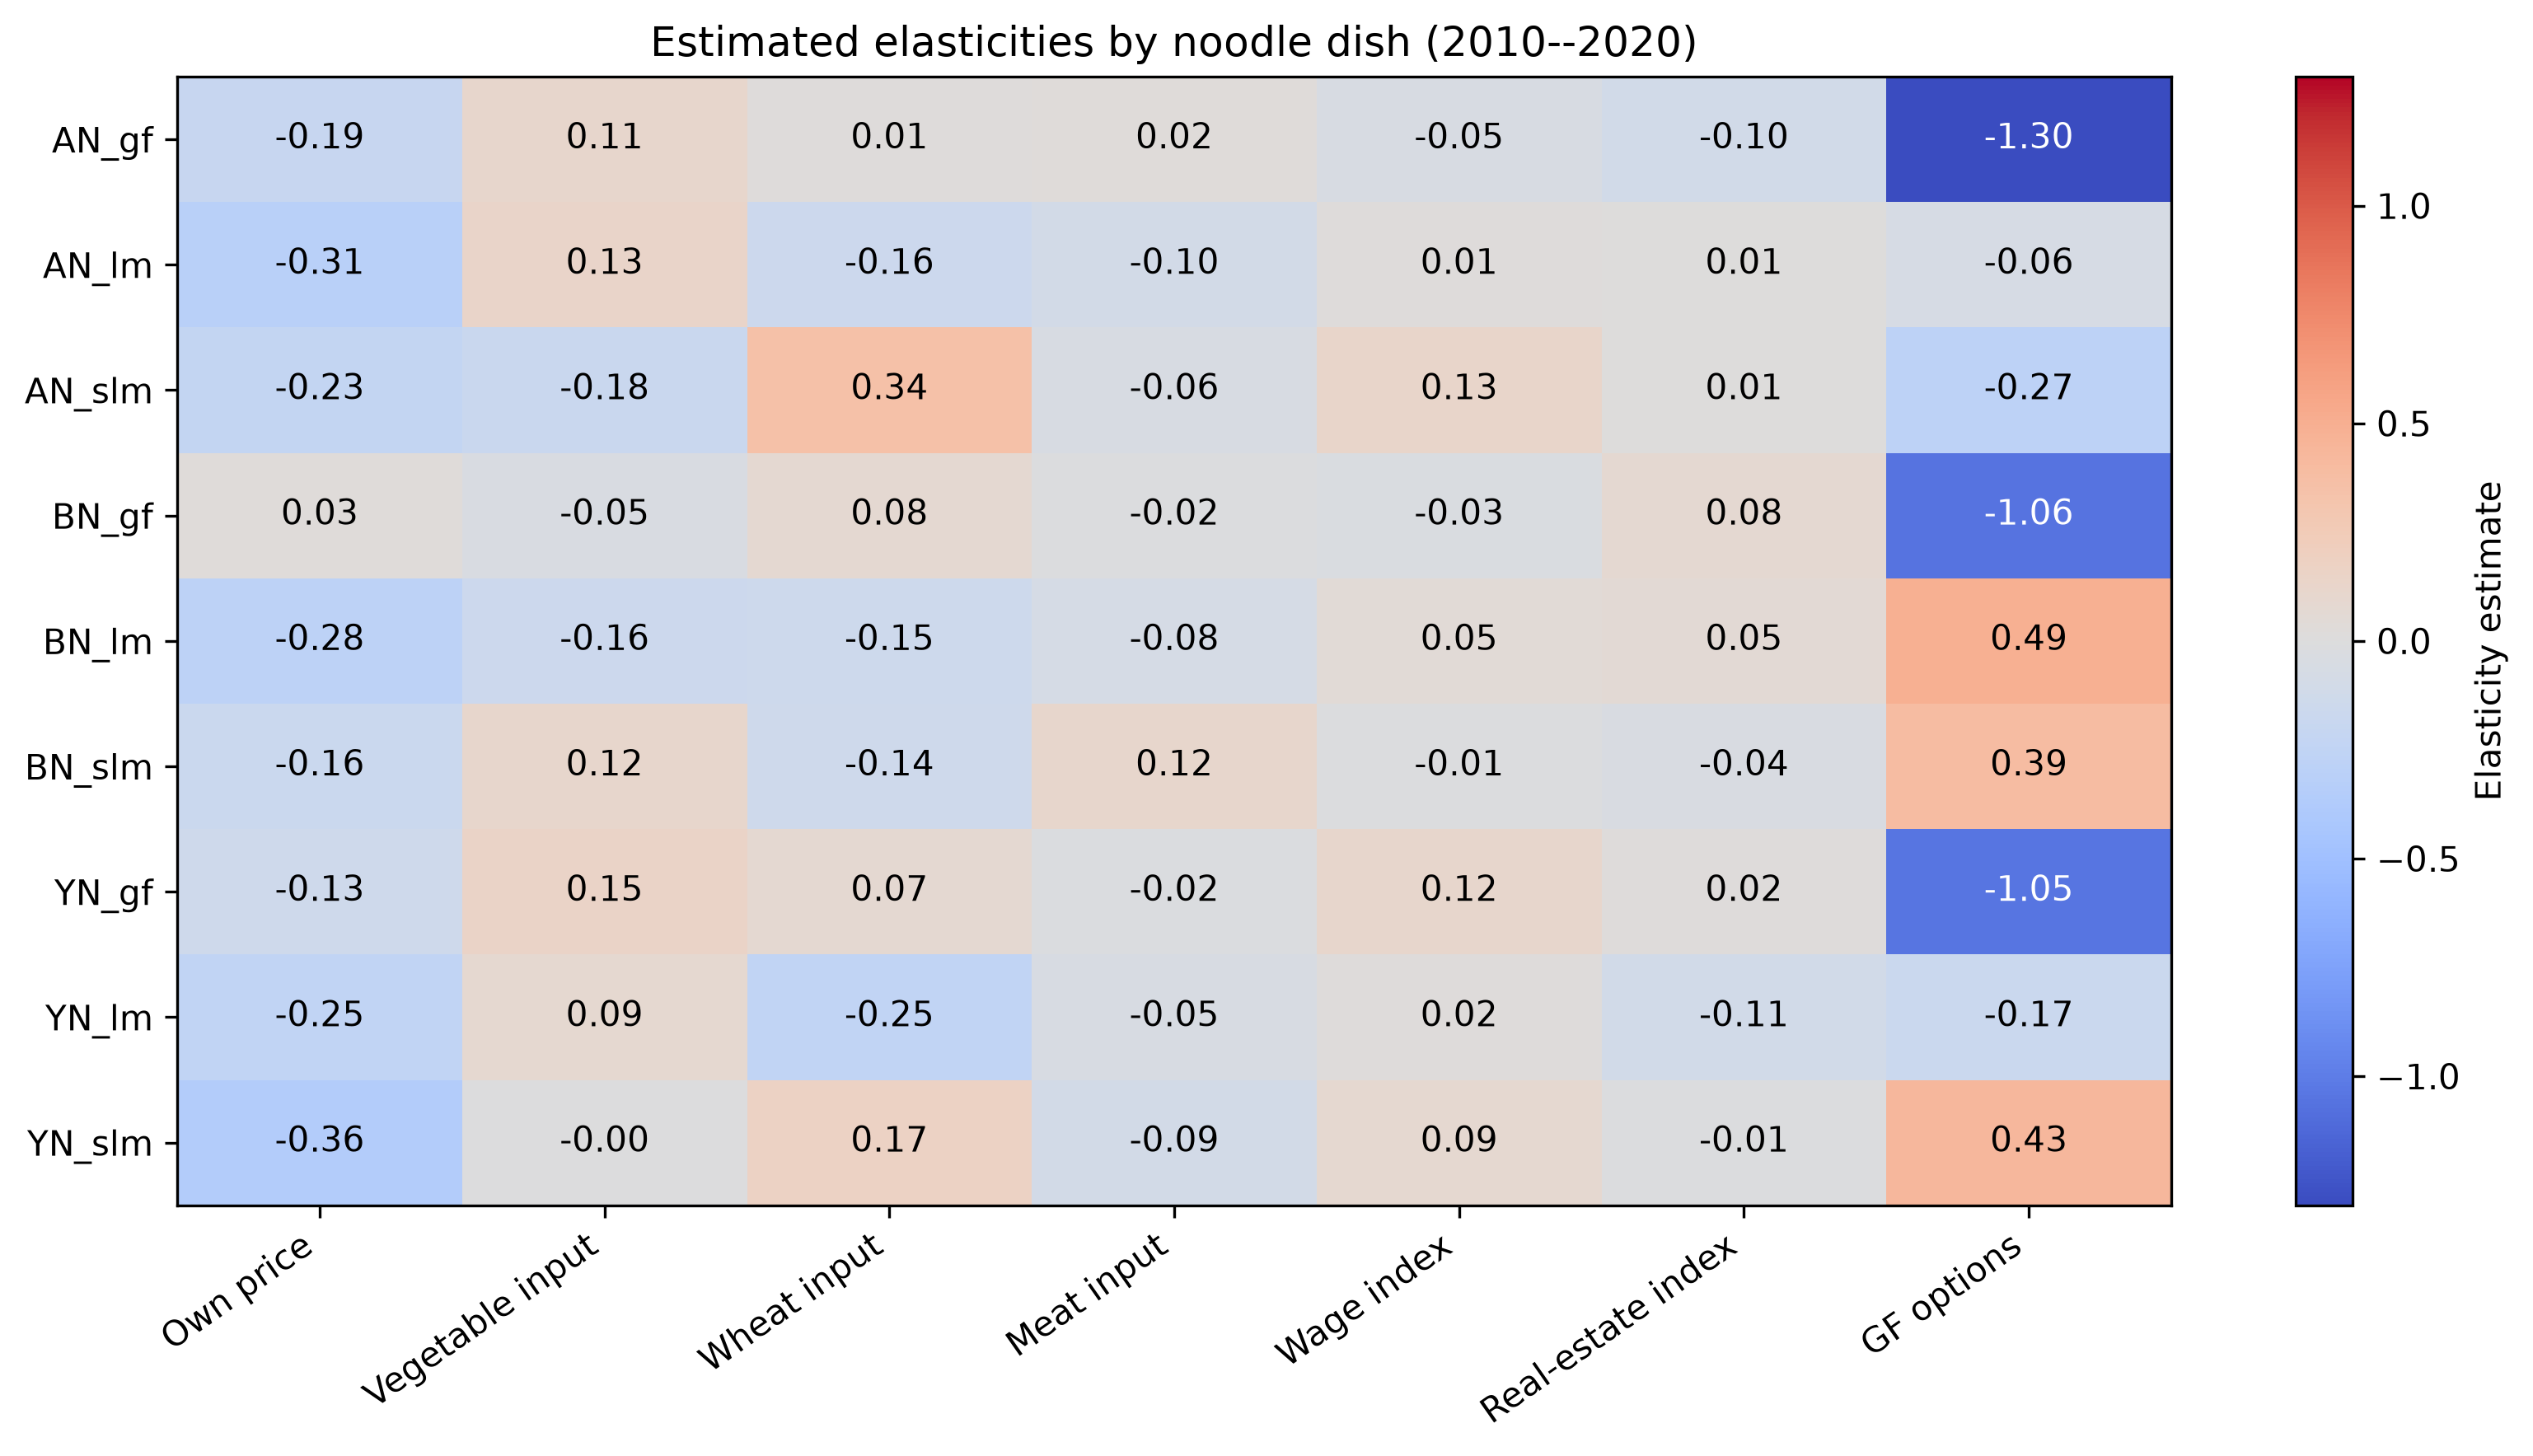
\includegraphics[width=0.9\linewidth,height=\textheight,keepaspectratio]{data/output/raw_elasticities.png}

}

\caption{\label{fig-raw-elasticities}Estimating Elasticities}

\end{figure}%




\end{document}
